%%%%%%%%%%%%%%%%%%%%%%%%%%%%%%%%%%%%%%%%%%%%%%%%%%%%%%%%%%%%%%%%%%% 
%                                                                 %
%                            CHAPTER FOUR                          %
%                                                                 %
%%%%%%%%%%%%%%%%%%%%%%%%%%%%%%%%%%%%%%%%%%%%%%%%%%%%%%%%%%%%%%%%%%% 

% EXPERIMENT COMMANDS
% ibeis -e rank_cdf --db humpbacks_fb -a default:has_any=hasnotch,mingt=2 -t default:proot=BC_DTW,decision=max,crop_dim_size=750,crop_enabled=True,manual_extract=True,use_te_scorer=True,ignore_notch=False,te_net=annot_res,te_score_method=avg,equalize_hist=False,kp_net=256_decoupled,tol=10 --dpath=/home/zach/data/results --save=<etc>.png --clipwhite

\chapter{Results} \label{sec:results}

In this chapter we present the results that our primary method achieves on the Flukebook dataset.
The main results for the optimal method are given briefly, and then we discuss how different variations on the method affect accuracy.
We go on to discuss the performance of our method when used in combination with Hotspotter.

\section{Main method}

The main method we settled on achieves an 80\% top-1 accuracy on the Flukebook dataset --- meaning that for 80\% of the query images, the correct identity is ranked first. 
The figures that we show in this section give the accuracy up to top-5 cumulatively.
In general we find that relative accuracies between configurations do not change significantly as we increase the rank at which we allow a match.
\\\\
The optimal configuration that we used for this method is given below.
\begin{itemize}
\item For every image, we predict keypoints by resizing a copy of the image to $128 \times 128$ and running it through the keypoint predictor.
\item Every image is then cropped between the predicted left and right tips, and resized to the same width ($750$ pixels) while maintaining aspect ratio. 
\item We do not use the bottom of the notch as a control point for trailing edge extraction.
\item We set the number of neighbors $n$ used in trailing edge extraction to $3$.
\item We use the Residual architecture for scoring the trailing edge.
\item The trailing edge score is averaged with the normalized gradient (i.e.\ $\beta = 0.5$).
\item We use $M =$ [2\%, 4\%, 6\%, 8\%] for our curvature scales.
%\item We weight all curvature scales equally
\end{itemize}


\section{Implementation}

All experiments in this thesis were carried out on a custom-built machine with a 6-core Intel i7 clocked at 3.5GHz, 64GB of RAM, and two nVidia GeForce GTX Titan X GPUs (each with 12GB of RAM). 
We make heavy use of numpy \cite{van2011numpy}, Theano\footnote{This allows for seamless switching between GPU and CPU computation} \cite{bergstra+al:2010-scipy, Bastien-Theano-2012}, and Lasagne \cite{sander_dieleman_2015_27878} for implementing our convolutional networks.
While most of the implementation is done in Python, we use C++ with Eigen \cite{eigenweb} for some of the core algorithms, namely trailing edge extraction, block curvature computation, and dynamic time warping.  

\section{Running Time}

%In this section, we discuss the wall-clock time of our method, as well as opportunities to improve it.

\begin{table*}[t]%
	\centering
	\resizebox{\linewidth}{!}
	{
		\begin{tabular} {| l || l | l | l | l || l |}
		\hline
		Stage & Keypoint Pred. & TE Scoring & TE Extraction & Block Curv. & Pairwise DTW \\
		\hhline{|=#===#==|}
		Time (ms) & 8.8 & 39.2 & 11.6 & 2.4 & 1.2 \\
		\hline
		\end{tabular}
	}
	\caption{\textbf{Itemized Running Time}. This table provides the average time taken for each operation that constitutes our algorithm on a single image. All computations were done on the subset of Flukebook that we used for evaluation (942 images).}
	\label{tab:extract_te_times}
\end{table*}




\subsection{Extracting Trailing Edges}
% 8 ms for KP prediction in batches of size 32
% 85 ms for TE scoring
% 11 ms for TE extraction
% 2 ms for block curv
% 1.2 ms for each comparison, so for a whole query we have 942*1.2ms = 1.1s

Table \ref{tab:extract_te_times} shows the times for each of these four stages.
There are four major stages in extracting a trailing edge that take a significant amount of time.
The first step is to predicting the fluke keypoints, the speed of which is largely dependent on the GPU used to run the convolutional network\footnote{A CPU could also be used but we do not test this here, and it would be significantly slower}.
In order to predict the keypoints faster we can ``batch'' the images before sending them to the GPU, which reduces communication overhead and better takes advantage of the GPU's massive parallelization capabilities.
The next step that takes a considerable amount of time is the trailing edge scoring.
This particular step is dependent on the size of the image, and is generally slow as the network is applied multiple times throughout the image.
Since each image is of a slightly different size we do not batch them, although this could be done with careful implementation.
For this analysis we only look at the Residual architecture, which is the slowest architecture evaluated.
Trailing edge extraction and block curvature computation take considerably less time, making the total time to go from image to curvature sequence 62ms per image.

Notably these computations were performed on our machine which has a considerably powerful GPU for its day.
As such, we would not expect the convolutional networks (particularly the trailing edge scorer) to perform similarly on a less powerful GPU.
These steps are of course be cached and reused for every image, so our matching algorithm's speed is independent of these times.


\subsection{Matching Trailing Edges}

We use a sequential search with no lower bounds to find a match for a given query in this work.
As such, for a given query our algorithm scales linearly in the size of the dataset that the query is to be matched against.
Given that the time for a single pairwise comparison between two computed curvatures (with our selected crop size and Sakoe-Chiba bound) is 1.2ms (Table \ref{tab:extract_te_times}), with our database of 942 images it takes just over one second to find a matching fluke.
Since we are doing a one-to-one comparison, our identification algorithm is embarrassingly parallel, providing an easy target for speed improvements.

\section{Configuration Options}

\subsection{Variability in Matching Score}

\begin{figure*}[t]%
\centering
\includegraphics[width=1\textwidth]{../images/results/score_sep_crop.png}
\caption{\textbf{Score Separability Histogram}. The blue bars in this figure represent true matches, and the red bars represent false matches. The line at $\text{score} = 0.88$ represents the optimal threshold at which to accept a match, although we can see it is not perfect.}
\label{fig:score_sep}
\end{figure*}

We find that a major issue with our method is the lack of strong correlation between the distance between two trailing edges and whether or not they belong to the same individual.
We can see this in Figure \ref{fig:score_sep}, which shows that the scores\footnote{The score is computed as $e^{\frac{-\text{distance}}{50}}$ for implementation reasons} between query trailing edges and their corresponding ground-truth trailing edge overlaps heavily with the distance between these queries and unrelated trailing edges.
The result of this is that small changes in the query and database trailing edges can (in some cases) cause the ranking of a ground-truth trailing edge to change significantly.
While this effect is rare given all of the queries, we find that it is the cause of many discrepancies in matching accuracy between different configurations.
With this in mind, we discuss the difference in matching accuracy only when it is a result of significant discrepancies --- meaning that the score between query and ground-truth trailing edge changes by more than $\epsilon = 0.02$ for a significant percentage of the match failures when two configuration options are compared.
We chose this value based on the score separation in Figure \ref{fig:score_sep}. 

\subsection{Effectiveness of Keypoint Extractor}
\begin{figure*}[t]%
\centering
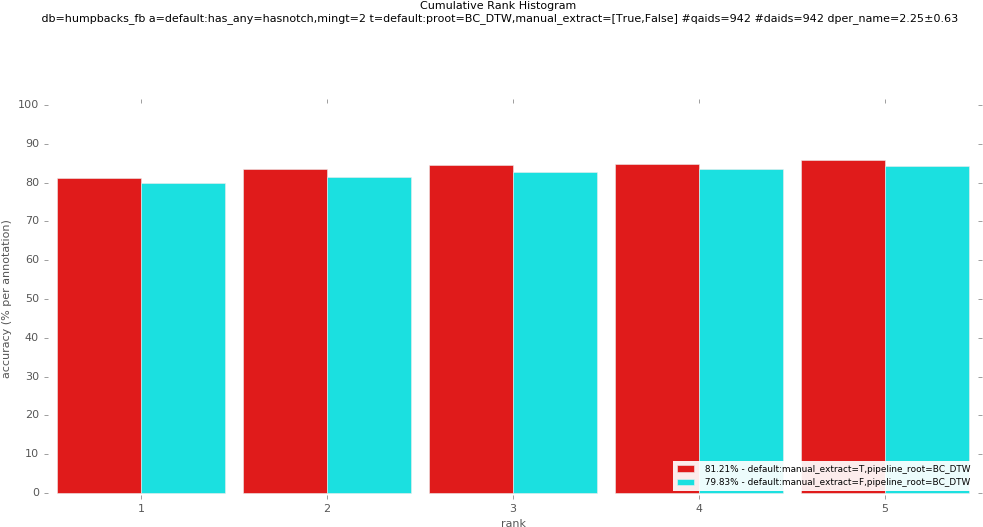
\includegraphics[width=1\textwidth]{../images/results/vary_manual_extract.png}
\caption{\textbf{Varying Manual Extraction}. There is a small difference in matching accuracy between using the manually annotated points (red) provided for this dataset versus the keypoint extractor's predicted points (cyan). The bottom of the notch keypoint is not used in these evaluations.}
\label{fig:vary_manual_extract}
\end{figure*}

In order to test the effectiveness of the trained fluke keypoint predictor, we give a comparison of matching accuracy against manual annotations of fluke keypoints\footnote{Provided with the Flukebook dataset} in Figure \ref{fig:vary_manual_extract}.
While this does not mean that the keypoints predicted are perfect, it does imply that they are ``good enough'' to extract a matchable trailing edge, despite being on average $5$ to $10$ pixels off.
Additionally, we found that only a small percentage of the match failures caused by automatic keypoint prediction were a result of differences in score above $\epsilon$.

%\subsubsection{Keypoint Extractor Image size}

%When predicting keypoints in an image, it is intuitive that the bigger the image the better the prediction can be, but at the expense of requiring more parameters (and thus memory, performance, and model variance) to handle the input.
%We can see in Figure \ref{fig:vary_kp_size}

%The primary difference between the networks that were trained to handle different size inputs is that, in order to ensure that all inputs to the final dense layers have the same spatial size ($2\times2$) across the different networks, an extra convolutional and pooling layer is added.

%\begin{figure*}[t]%
%\centering
%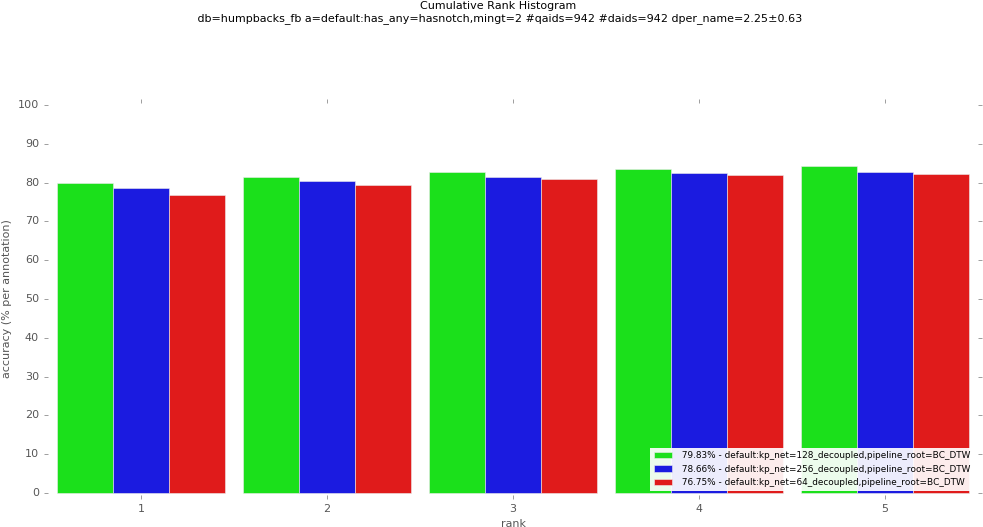
\includegraphics[width=1\textwidth]{../images/results/vary_kp_size.png}
%\caption{\textbf{Varying Keypoint Image Size}. The larger keypoint image size provides a somewhat better accuracy. We did not see an improvement in accuracy beyond an image sizee of $128 \times 128$.}
%\label{fig:vary_kp_size}
%\end{figure*}

%We trained each of these networks on separate splits of data, and due to the inherent stochasticity of the training it is difficult to ascertain whether or not the image size is a cause of performance issues. 

%\subsubsection{STN} % Maybe?

%We also briefly experimented with an Spatial Transformer Network \cite{jaderberg2015spatial}.
%This was largely motivated by the tendency of the keypoint extractor to poorly predict fluke keypoints on flukes that did not ``fill'' the image horizontally.
%Unfortunately, we could not get the STN to converge at a better accuracy than the standard keypoint extractor, even if we held its parameters fixed for a few training epochs.
%Usually, the STN would produce nonsensical transformations of the image.

\subsection{Cropping Width}


With dynamic time warping, we theoretically can match trailing edges of arbitrary lengths --- however the distances can be distorted by large differences in actual trailing edge length.
For this reason we fix the length of the trailing edges.
Since we are only interested in the width of an image (because of the way the trailing edge extraction algorithm works), we can get every trailing edge to have exactly some fixed length $w$ by the following process.

\begin{itemize}
    \item Crop the image horizontally between the left and right columns found by the keypoint extraction process (or manually determined).
    \item Resize the cropped image to some fixed width $w$ while preserving the aspect ratio.% using Lanczos interpolation. % Maybe find citation for this
\end{itemize}

\begin{figure*}[t]%
\centering
%\subfloat[Distribution of Image Widths][]{
%	\includegraphics[width=0.5\textwidth]{../images/results/chip_width_hist_fb.png}
%}
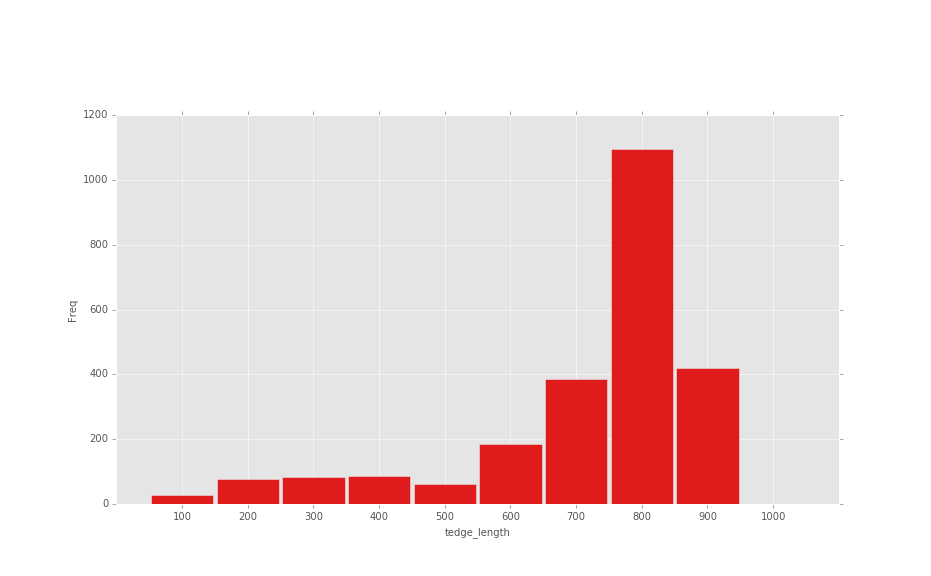
\includegraphics[width=1\textwidth]{../images/results/te_size_hist_fb.png}
\caption{\textbf{Distribution of Unresized Trailing Edge Lengths}. This shows a significant distribution of trailing edges centered around a width of 800 pixels.}
\label{fig:width_te_dist}
\end{figure*}

In this way, we standardize the trailing edge length so that differences in image size do not affect detection accuracy.
One major caveat with this process is of course that using the keypoint extractor's predictions can cause catastrophic failures in this process (e.g.\ if the left and right points are nowhere near a fluke), however in practice we found that this is not an issue.

%We can see in Figure \ref{fig:vary_crop_nocrop} that cropping and resizing is absolutely vital to the performance of our algorithm.

%\begin{figure*}[t]%
%\centering
%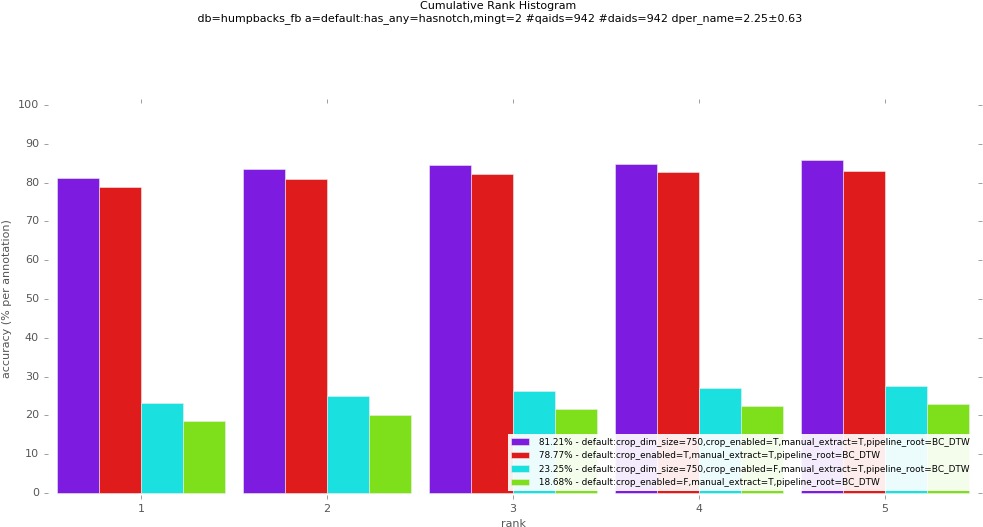
\includegraphics[width=1\textwidth]{../images/results/vary_crop_nocrop.png}
%\caption{\textbf{Varying Crop Strategy}. Cropping images around the trailing edge and then resizing them proves to be very important, not doing so gives a very low accuracy. We can see in Figure \ref{fig:chip_size_hist} that there is a wide distribution of image sizes, which can hamper the effectiveness of DTW.}
%\label{fig:vary_crop_nocrop}
%\end{figure*}

%We also note that we originally tried histogram equalization as part of the preprocessing pipeline, although it produced significantly worse trailing edges (and subsequently matching accuracy).

Ideally, we would choose a $w$ that minimizes the interpolation artifacts that result from making big changes in image size.
Figure \ref{fig:width_te_dist} shows the histogram of post-crop widths (i.e\ trailing edge lengths) from unresized images in the Flukebook dataset, showing a large concentration of mass around 800 pixels. 
Subsequently, Figure \ref{fig:vary_crop_size} shows that $w = 750$ performs well, although $w = 1000$ is on par.
We select the former for efficiency's sake, as smaller trailing edges vastly improves the speed of the matching algorithm.
This provides evidence for the hypothesis that the less the image has to be resized, the better the trailing edge.

%\subsection{Trailing Edge Extraction}

%One major result that we found was that, when using the averaging method to combine the trailing edge scores with $N_y$, having a robust trailing edge prediction wasn't as important as having a detailed trailing edge.

\begin{figure*}[t]%
\centering
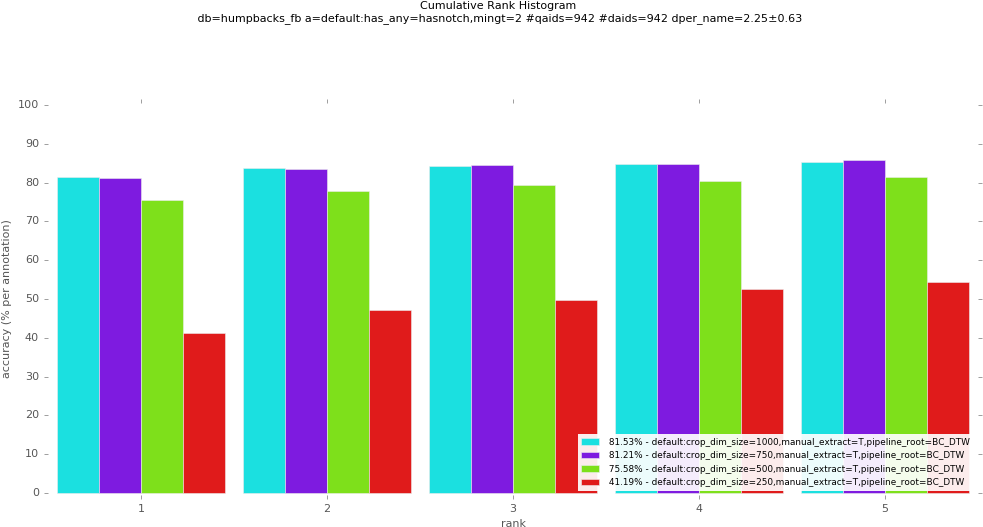
\includegraphics[width=1\textwidth]{../images/results/vary_crop_size.png}
\caption{\textbf{Varying $w$}. Note that we use the manually annotated points in this analysis to control for any issues with keypoint extraction.}
\label{fig:vary_crop_size}
\end{figure*}


\subsection{Trailing Edge Scorer Architecture}

The various trailing edge scorer architectures and their results on the task they were trained for is detailed in the previous chapter (see Table \ref{tab:te_score_full_analysis}).
In Figure \ref{fig:vary_te_scorer} we present the actual matching accuracies that each one produced with the mixing parameter $\beta = 0.5$.
We can see that the detailed and higher quality trailing edges produced by the Residual network give a decent performance boost over the other networks, however this performance boost appears to consist mostly of insignificant changes in query to ground truth distance.

\begin{figure*}[t]% \centering
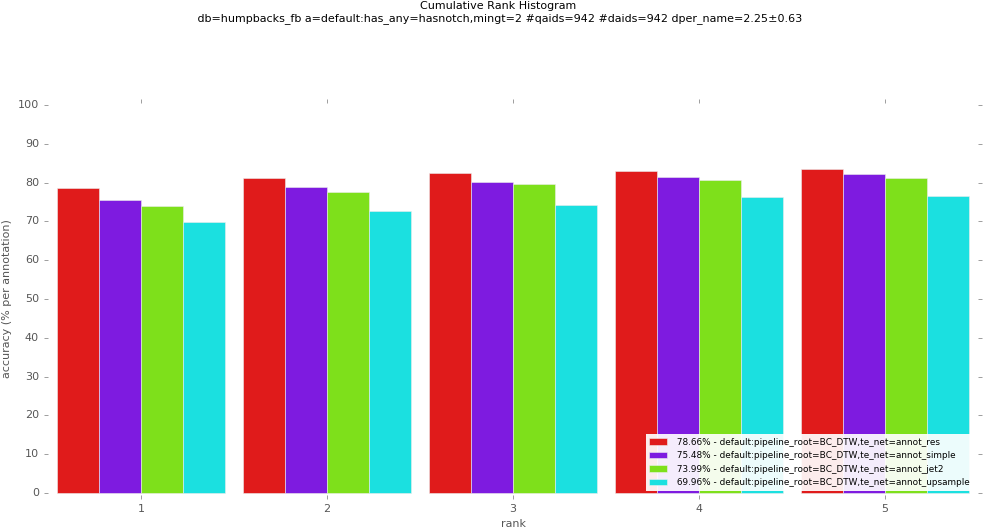
\includegraphics[width=1\textwidth]{../images/results/vary_te_scorer.png}
\caption{\textbf{Trailing Edge Scorer Architectures}. The highest performing trailing edge scorer (Residual) is shown in red, followed by Simple, Jet, and Upsample (in descending order of accuracy).}
\label{fig:vary_te_scorer}
\end{figure*}

A better evaluation of each trailing edge scoring architecture is given in Figure \ref{fig:vary_te_scorer_maxweight} where we only use the trailing edge scorer outputs to extract the trailing edge (i.e.\ $\beta = 1.0$).
Unsurprisingly, since the Upsample network gives blocky trailing edges (see Figure \ref{fig:te_upsample}), it performs very poorly.
One of the benefits we observed with the Upsample network is that it does not make the same amount of spurious trailing edge predictions that the other networks make.
However we can see that this is not as helpful as simply producing more fine-grained predictions.

\begin{figure*}[t]%
\centering
\includegraphics[width=1\textwidth]{../images/results/vary_te_scorer_maxweight.png}
\caption{\textbf{Trailing Edge Scorer Architectures at $\beta = 1$}. Upsample (cyan) performs significantly worse than the other networks, which all perform comparably.}
\label{fig:vary_te_scorer_maxweight}
\end{figure*}

One caveat with using the Residual network is that, with 64 layers, it consumes a lot of GPU memory to make a prediction.
This is currently an implementation issue, however the machine that we use for these experiments has the capacity to run the Residual network.
However, given that each network performs comparably, the Simple network is a good choice in general.

\subsection{Using a Trailing Edge Scorer}

In Figure \ref{fig:vary_te_weight}, we can see that simply a pixel-wise average of $N_y$ and $(1-T_y)$ (i.e. $\beta = 0.5$) produces the best results for the Residual network, though the differences are largely insignificant.
However, not using the trailing edge scorer (i.e.\ $\beta = 0$) performs significantly worse than using one at all (even with a low weight).
We show an example case where trailing edge scoring helps in Figure \ref{fig:dis_te_use}.

\begin{figure*}[t]%
\centering
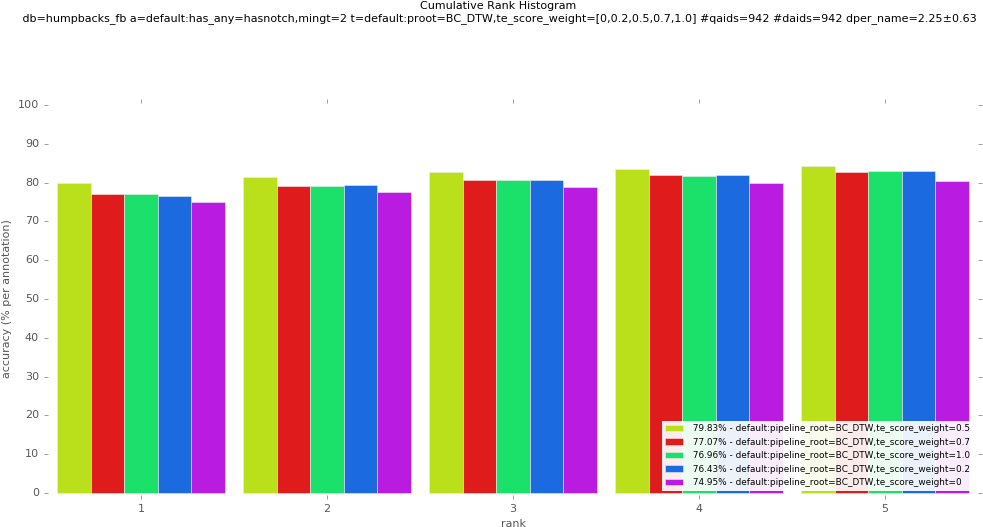
\includegraphics[width=1\textwidth]{../images/results/vary_te_weight.png}
\caption{\textbf{Varying $\beta$}. Setting $\beta = 0.5$ (yellow) provides only marginally better results over any other non-zero value of $\beta$, but is significantly better than $\beta = 0$ (purple).}
\label{fig:vary_te_weight}
\end{figure*}


\subsection{Number of neighbors in the extraction}

The number of neighbors $n$ effectively limits the slope of the trailing edge.
We limit it to an odd number for convenience.
On the one hand, a lower $n$ can cause the trailing edge to be limited in vertical breadth, but does prevent it from going way off course.
Despite this, with trailing edge scoring in place, it might be beneficial to increase $n$ so as to avoid parts of the trailing edge that continually ``max out'' the number of neighbors.

\begin{figure*}[t]%
\centering
\subfloat[][$\beta = 0.5$]{
	\includegraphics[width=0.5\textwidth]{../images/results/aid207_te_kp_overlay.png}
}
\subfloat[][$\beta = 0$]{
	\includegraphics[width=0.5\textwidth]{../images/results/aid207_te_kp_overlayno_tescorer.png}
}
\newline
\subfloat[][$T_p$]{
	\includegraphics[width=0.5\textwidth]{../images/results/aid207_tescorer_annot_res.png}
}
\subfloat[][$I_y$]{
	\includegraphics[width=0.5\textwidth]{../images/results/aid207_grad.png}
}
\caption{\textbf{Example Use of Trailing Edge Scorer}. In (a), we have the trailing edge extracted with the Residual scorer. Compare to (b), which did not use any scorer at all, resulting in a match failure.}
\label{fig:dis_te_use}
\end{figure*}

Ultimately, we can see in Figure \ref{fig:vary_neighbors} that limiting the number of neighbors to the immediate neighborhood (i.e. $n = 3$) produces a significant boost over a larger neighborhood.
We hypothesize that the trailing edges extracted with $n = 3$ are necessarily less detailed, and as a result can be more invariant to slight changes in pose of the fluke.
%Figure \ref{fig:dis_neighbors} presents an example case where, when using a higher number of neighbors, the notch is captured more faithfully --- but this introduces differences between the query and ground truth trailing edges that impede matching.
While this effect is only present in a small number of cases, the difference in accuracy here is significant, with 78\% of the improvements resulting in a score difference over $\epsilon$.

\begin{figure*}[t]%
\centering
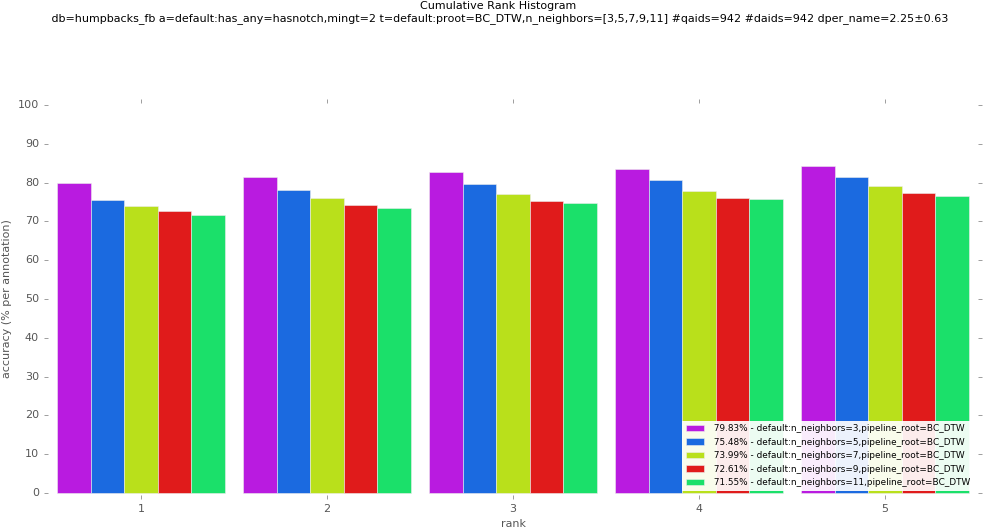
\includegraphics[width=1\textwidth]{../images/results/vary_neighbors.png}
\caption{\textbf{Varying $n$}. This shows that the optimal neighborhood constraint is $n = 3$ (purple), despite qualitatively producing worse-looking trailing edges. After $n = 5$ (blue), the trailing edges can become very noisy affecting match accuracy.}
\label{fig:vary_neighbors}
\end{figure*}

\subsection{Using the notch}

Initially, we believed that using the notch as a control point (i.e.\ forcing the trailing edge to go through the notch) would give better trailing edges, and therefore an increase in accuracy.
As it turns out, this is not the case --- using the notch as a control point gives somewhat worse accuracy.
Surprisingly, this decrease in matching accuracy holds for both manually annotated and automatically extracted keypoints.
However, most of these discrepancies did not result in a score difference above $\epsilon$.
This could be because of the small difference in trailing edge between those with the notch as a part of the trailing edge and those without, which leads to matching failure but not a large difference in score.

%\begin{figure*}[t]%
%\centering
%\includegraphics[width=1\textwidth]{../images/results/vary_ignore_notch.png}
%\caption{\textbf{Using the notch as a control point}. Ignoring the notch point (cyan) gives better accuracy than using the notch point (red).}
%\label{fig:vary_notch}
%\end{figure*}

\subsection{Curvature Scales}

Computing the curvature is one of the least parameterized parts of the process.
Despite this, figuring out what the optimal scales (and how many) are is expensive to do experimentally.
Instead of exhaustively exploring these options, we use heuristics to determine which curvature scales to explore.
Each scale measures the curvature of some percentage of the trailing edge around each point on the trailing edge.
Intuitively, we want to capture the curvature at a scale that provides the most variation between trailing edges.
Therefore, in order to determine which scales to measure, we look at how much the actual curvature changes between successive scales, as well as the average variance in curvature among trailing edges at each scale. 

\begin{figure*}[t]%
\centering
\subfloat[][Curvature Diversity]{
	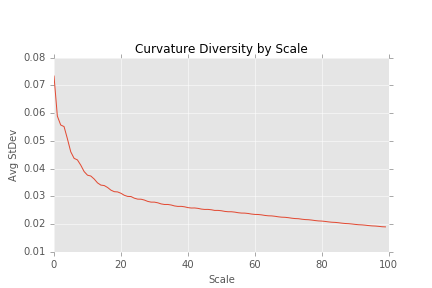
\includegraphics[width=0.5\textwidth]{../images/results/curvature_diversity_fb.png} 
	\label{fig:curvature_diversity:a}
}
\subfloat[][Inter-scale difference]{
	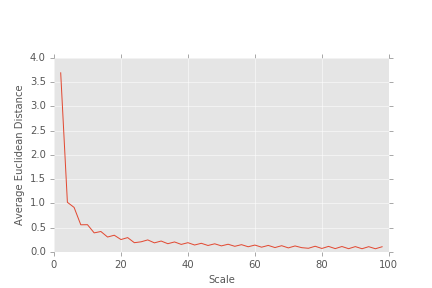
\includegraphics[width=0.5\textwidth]{../images/results/interscale_diff_fb.png} 
	\label{fig:curvature_diversity:b}
}%
\caption{\textbf{Curvature Diversity}. Left panel (a) shows the average standard deviation of the (fixed length) curvature at different scales. Right panel (b) shows the average Euclidean distance between curvatures measured at successive scales.}
\label{fig:curvature_diversity}
\end{figure*}

We find that (Figure \ref{fig:curvature_diversity:a}) as block curvature scale is increased, the diversity at any given point in the curvature goes down drastically (as expected). 
Therefore, we stick to the lower end of the scale, keeping the curvature scales measured below $10\%$.
We can also see in Figure \ref{fig:curvature_diversity:b} that successive curvature scales show bigger differences at lower scales than at higher scales, which reinforces using curvatures below $10\%$, but also encourages bigger jumps between scales to maximize diversity while minimizing computation time.
Based on the above, we evaluated scales that run from $1\%$ to $10\%$, with varying levels of resolution, and found little to no significant effect on matching accuracy compared to using the default set of scales.

%\begin{figure*}[t]%
%\centering
%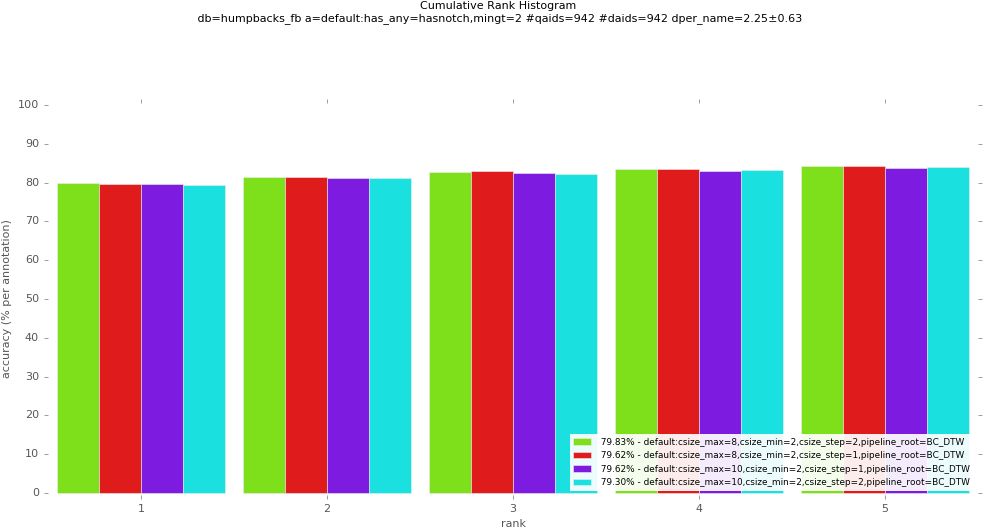
\includegraphics[width=1\textwidth]{../images/results/vary_curv_scales.png}
%\caption{\textbf{Varying Curvature Scales}. The scales evaluated here are parameterized with a start, end, and step size. We always start at 2\%, and vary the step size between 1 \& 2 and the end between 8\% \& 10\%.}
%\label{fig:vary_curv_scales}
%\end{figure*}

\subsection{Sakoe-Chiba bound}

%The main variants shown in this section are the different Sakoe-Chiba bound windows and the scale weighting term in the curvature distance function.

%\subsubsection{Weighting the different scales}

%There are many ways to produce the weights $s_w$ for curvatures, but intuitively there should be a monotonic relationship between curvature scale and importance.

%We could specify this relationship as a ratio $W$ of importance between successive pairs of curvatures (increasing in size).
%We parameterize that importance by giving each scale the weight $s_w = [W^i \forall i \in [0,|S|]$.
%In order to maintain this ratio without blowing up the distances, we also normalize so that $\sum s_w = 1$.

%\begin{figure*}[t]%
%\centering
%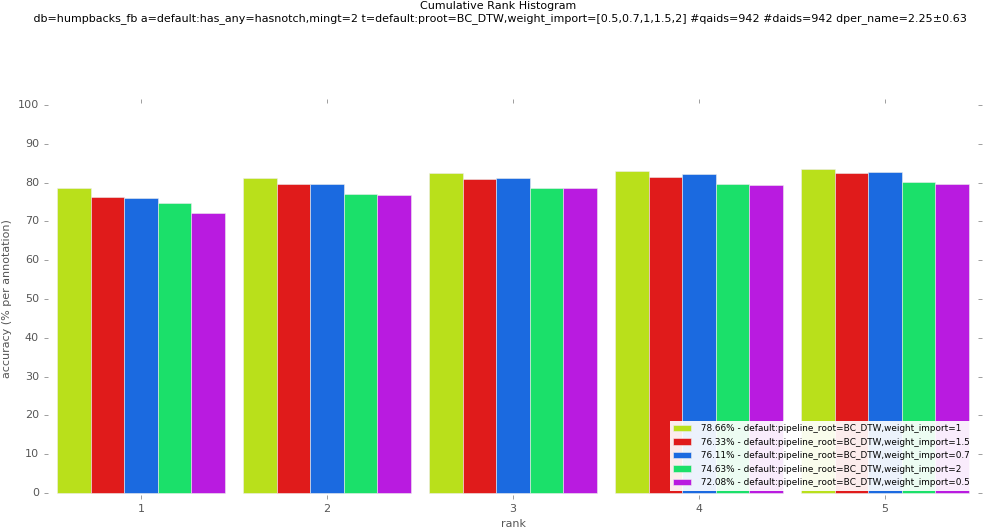
\includegraphics[width=1\textwidth]{../images/results/vary_weight_import.png}
%\caption{\textbf{Varying $s_w$}. The yellow bar shows $W = 1$, i.e.\ all curvatures weighted equally.}
%\label{fig:vary_weight_import}
%\end{figure*}



%Figure \ref{fig:vary_weight_import} shows that despite this effort, it appears that equally weighting each curvature scale provides the best performance.
%Interestingly weighting larger scales lower (i.e.\ $W < 1$, which we evaluate with $W = 0.5$ (purple bar) in Figure \ref{fig:vary_weight_import}) provides worse performance.

\begin{figure*}[t]%
\centering
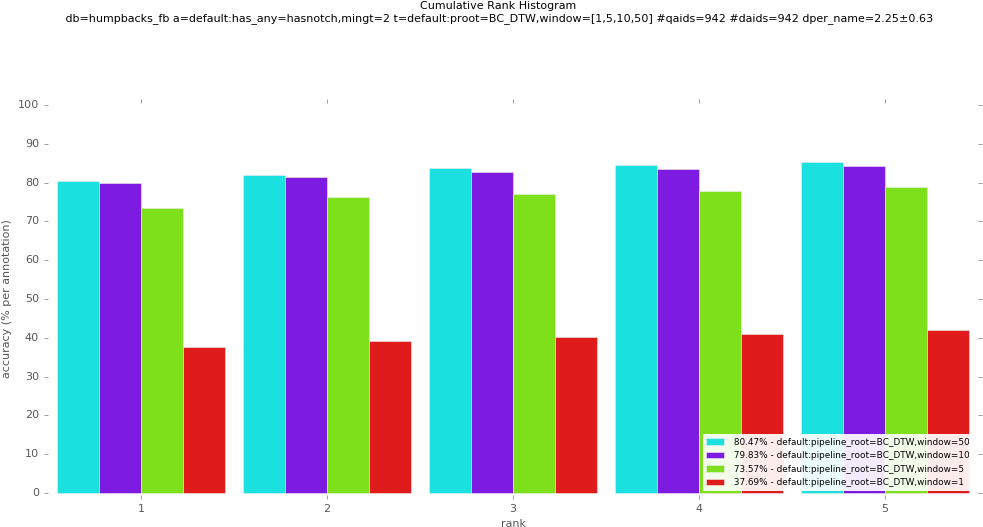
\includegraphics[width=1\textwidth]{../images/results/vary_window.png}
\caption{\textbf{Varying Sakoe-Chiba Bound}. We achieve good results with the Sakoe-Chiba bound set to $10\%$ (yellow), although we can get slightly better results with it set to $50\%$ (green) at the expense of computation time.}
\label{fig:vary_window}
\end{figure*}



In Figure \ref{fig:vary_window}, we show the effects of varying the window (i.e.\ the Sakoe-Chiba bound $T$) in the dynamic time warping distance computation.
At around 10\% of the query trailing edge length we maintain only slightly worse accuracy compared to the full window (i.e.\ 50\%), but below this accuracy is severely affected.
We find that overall there is a $4\times$ slow-down in wall-clock time on our testing machine when going from a window size of 10\% to one of 50\%. 
Thus, we use this value for the window size so as to minimize computation time while maintaining the total accuracy.
Additionally, while it is possible for gross mismatches to occur from there being no window boundary, we can see from Figure \ref{fig:vary_window} that this does not pose a problem.

%\subsubsection{Aggregating over multiple trailing edges per identity}

%Determining the identity of a given query image given distances to other images in the database is not entirely simple when there are multiple database images for a given individual.
%Essentially we need to transform these distances from query image to database image into distances from query to known individual.
%To do so we evaluate two options given a group of distances for an individual --- either the average distance or the minimum distance.

%We find that the average decision does slightly better, as shown in Figure \ref{fig:vary_decision}.

%This is unsurprising given that most of the individuals in the dataset only have two images associated, meaning that the average is equivalent to the minimum.
%That said, the minimal distance criterion is effectively the single-feature case of LNBNN used in Hotspotter \cite{crall_hotspotter_2013} and the work of Hughes et al.\ \cite{hughes2015automated}. % Maybe: prove this?

%\begin{figure*}[t]%
%\centering
%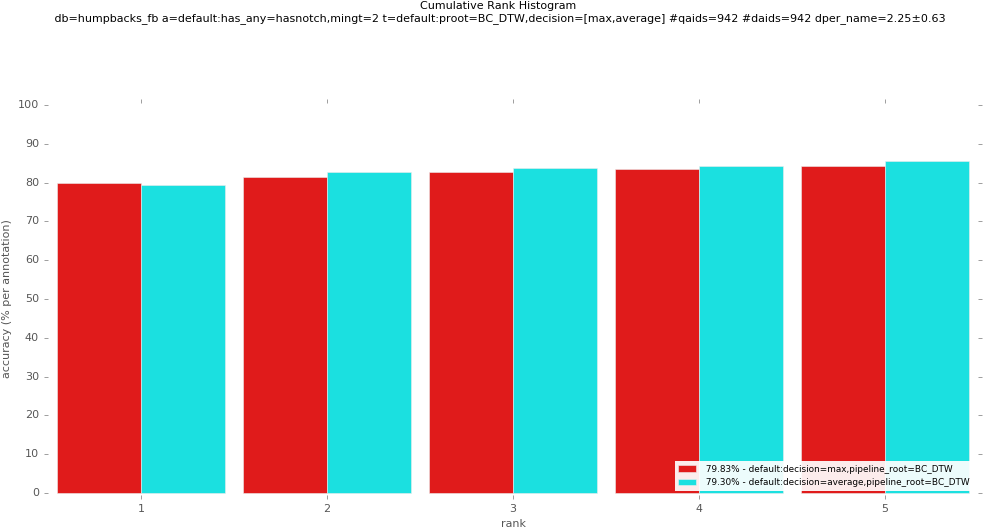
\includegraphics[width=1\textwidth]{../images/results/vary_decision.png}
%\caption{\textbf{Varying Decision Criterion}}
%\label{fig:vary_decision}
%\end{figure*}

\section{In Combination with Hotspotter}

\begin{figure*}[t]%
\centering
\subfloat[][Query Image 1]{
	\includegraphics[width=0.5\textwidth]{../images/results/aid493_te_kp_overlay.png}
}
\subfloat[][Correct Match 1]{
	\includegraphics[width=0.5\textwidth]{../images/results/aid147_te_kp_overlay.png}
}
\newline
\subfloat[][Query Image 2]{
	\includegraphics[width=0.5\textwidth]{../images/results/aid494_te_kp_overlay.png}
}
\subfloat[][Correct Match 2]{
	\includegraphics[width=0.5\textwidth]{../images/results/aid148_te_kp_overlay.png}
}
\caption{\textbf{Example Disagreements Between Hotspotter and our method}. On the left side, (a) was matched correctly to (c) by our method, whereas Hotspotter could not find any matches for (a). On the right hand side however, Hotspotter gave (d) as the top match for (b) despite a large variance in pose and lighting, while our method failed to rank (d) in the top 5 matches for (b).}
\label{fig:dis_proot}
\end{figure*}

Comparatively, our method gets a slightly better top-1 accuracy than Hotspotter (see Table \ref{tab:vary_proot}).
However, our method targets a specific part of the fluke whereas Hotspotter recognizes general patterns, and thus can make use of the internal texture of the fluke.
Therefore, by combining our method with Hotspotter --- if we were able to automatically pick out which algorithm was right for a given ranking --- we would expect to see a significant increase in accuracy.
We find that in this ideal scenario, we can achieve a 93\% top-1 accuracy on the Flukebook dataset.
However, automatically deciding which algorithm to use for matching is non-trivial, and we are still exploring it.

See Figure \ref{fig:dis_proot} for an example where Hotspotter correctly finds a match where our method fails, and vice-versa.

\subsection{Characterization of when to use which method}

From an intuitive standpoint, it appears that Hotspotter cannot find effective keypoints from trailing edges, which hampers its ability to handle flukes which do not have an apparent pattern.

We hypothesize that this is because the trailing edge --- while a distinctive feature --- inevitably shares a region with an oceanic background.
Since this oceanic background changes from image to image, it cannot verify salient keypoints as matches.
As a result, flukes which have little to no internal texture are nearly impossible for Hotspotter to match.

\begin{table*}[t]%
	\centering
	\resizebox{\linewidth}{!}
	{
		\begin{tabular} {| l || l | l | l |}
		\hline
		Method & Hotspotter & Our Method & Hotspotter $\cup$ Our Method \\
		\hhline{|=#===|}
		Top-1 Accuracy  & 77.81\% & 79.83\% & 93.52\% \\
		\hline
		\end{tabular}
	}
	\caption{\textbf{Comparison with Hotspotter}. This table provides a comparison between our method and Hotspotter in terms of top-1 ranking accuracy on the Flukebook dataset.}
	\label{tab:vary_proot}
\end{table*}




%\begin{figure*}[t]%
%\centering
%\includegraphics[width=1\textwidth]{../images/results/vary_proot.png}
%\caption{\textbf{Comparison between Hotspotter and our method}. Hotspotter's accuracy (cyan) is slightly worse than our method's (red), however we find that they are fairly complementary. Note that Hotspotter's accuracy does not increase much with allowed matching rank.}
%\label{fig:vary_proot}
%\end{figure*}



On the other hand, when the trailing edge is unclear or significantly distorted in the image, our method struggles to find an appropriate match.
In these cases, Hotspotter can provide a good match, although if the fluke is additionally untextured we have an issue.
We were unable to find a single heuristic that correlates with our method failing to find a match.
Particularly we find that smoothness of the trailing edge, characterized by the standard deviation of the trailing edge slope, does not correlate to match failure.
This implies that smooth trailing edges are about as easy to match for our method as rough, distinctive trailing edges.
However, since the dataset we use consists primarily of individuals with only two images, there is necessarily a lot of variation in ``matchability'' of given pairs of images.


%%% Local Variables: 
%%% mode: latex
%%% TeX-master: t
%%% End: 
